\documentclass[tikz]{standalone}
\usepackage{pgfplots}
\pgfplotsset{compat=1.15}
\usepackage{mathrsfs}
\usetikzlibrary{arrows,calc}
\usepackage{tkz-euclide}
\pagestyle{empty}

\definecolor{AngleClr}{rgb}{0,0.39215686274509803,0}
\definecolor{ShapeClr}{rgb}{0.6,0.2,0}
\definecolor{SquareClr}{RGB}{250, 248, 217}

\usepackage{fp}
\usepackage{xfp}

\begin{document}

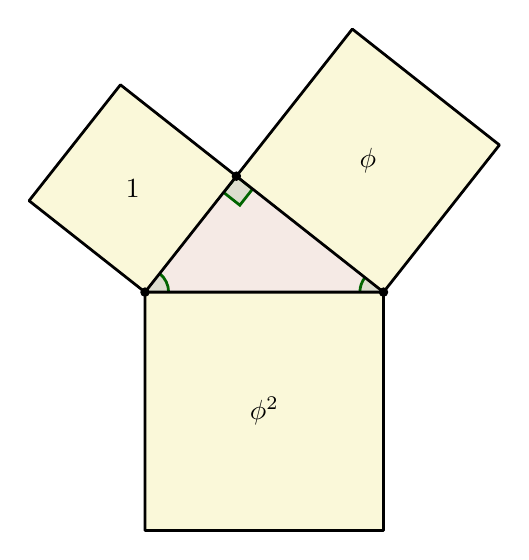
\begin{tikzpicture}[scale=.75]
\tkzSetUpLine[line width=1pt,color=black]
\tkzSetUpPoint[fill=black]

\def\Scale{2.5}
\def\La{1 * \Scale}
\def\Lb{1.26885775 * \Scale}
\def\Lc{\fpeval{sqrt(\La * \La + \Lb * \Lb)}}

\FPeval{\Ax}{\La * \La / \Lc}
\FPeval{\Ay}{\La * \Lb / \Lc}

\tkzDefPoints{0/0/B,\Ax/\Ay/A,\Lc/0/C}


\tkzFillPolygon[fill=ShapeClr,fill opacity=0.1](A,B,C)
\tkzMarkRightAngle[line width=1pt, size=.35,color=AngleClr,fill=AngleClr,fill opacity=0.1](B,A,C)
\tkzFillAngle[fill=AngleClr,size=.4,fill opacity=0.1](C,B,A)
\tkzMarkAngle[line width=1pt,size=.4,color=AngleClr](C,B,A)
\tkzFillAngle[fill=AngleClr,size=.4,fill opacity=0.1](A,C,B)
\tkzMarkAngle[line width=1pt,color=AngleClr,size=.4](A,C,B)

\tkzDefSquare(B,A)\tkzGetPoints{AA}{AB}
\tkzDrawPolygon[fill=SquareClr](A,B,AB,AA);

\tkzDefSquare(A,C)\tkzGetPoints{CA}{CC}
\tkzDrawPolygon[fill=SquareClr](A,C,CA,CC);

\tkzDefSquare(C,B)\tkzGetPoints{BC}{BB}
\tkzDrawPolygon[fill=SquareClr](B,C,BB,BC);

\tkzDefMidPoint(CC,C) \tkzGetPoint{MC}
\tkzDefMidPoint(BB,B) \tkzGetPoint{MB}
\tkzDefMidPoint(AB,A) \tkzGetPoint{MA}

\tkzLabelPoint[anchor=center](MA){$1$}
\tkzLabelPoint[anchor=center](MB){$\phi^2$}
\tkzLabelPoint[anchor=center](MC){$\phi$}

\tkzDrawPoints[size=3](A,B,C)

\end{tikzpicture}

\end{document}
